
Verifying game theoretic properties in protocols has become very important and tricky because, the original definitions of game representations and the generic algorithms to find the Nash equilibriums do not help a lot in optimizing protocol verification. As mentioned in the previous section, model checking research community strongly focuses on application and property specific optimizations. Developing model checking algorithms to verify game theoretic properties is very useful under this background. 
\newline
On the other hand, some real world protocols are easy to analyse when they are represented as games. Following section provides some examples of using model checking to verify game theoretic properties.
\newline

\section{APPLICATIONS OF MODEL CHECKING FOR GAME THEORY}

Contract signing protocols have game-like properties that can be verified by model checking. A two-party contract is an exchange agreement.Informally, if both parties perform the contract, they have some utility. If one party violates the contract, the violator gets more utility and the other party receives less. It is evident that designing a simultaneous contract signing protocol which is fair, without either a trusted third party or a partial commitment scheme is usually difficult in practice.\cite{Ben-Or1990} A simple example for a partial commitment scheme is as follows.

\begin{figure}[H]
	\centering
	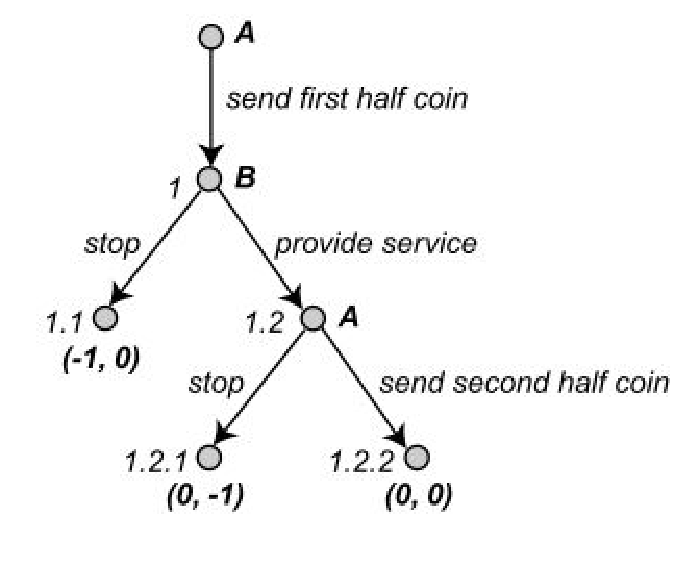
\includegraphics[width=\textwidth]{non_zero_sum3}
	\caption{Exchange Example}
	\label{fig:contract_example}
\end{figure}

 Figure \ref{fig:contract_example} \cite{Buttyan1999} defines a protocol in which player $A$ sends a half coin before player $B$ provides the service. If player $B$ provides the service, player $A$ can send the other half of the coin. If player $B$ does not provides the service, player $A$ gets a negative reward, because he lost half a coin and he has another half of a coin which he can't use. If player $A$ does not send his first half of the coin, protocol does not proceed and both players have no loss nor gain. The utilities for $A$ and $B$ are shown within brackets. This is exactly an example for an extensive game with perfect information. A similar example about a certified email protocol is mentioned in \cite{Buttyan1999}. \newline
 Probabilistic protocols for contract signing introduces parameters quantify fairness. Rabin's protocol\cite{Rabin83} and BGMR protocol\cite{Ben-Or1990} are two such probabilistic contract signing protocols. Following are the major steps of Rabin's protocol.
 
 \begin{algorithm}[H]
 	\floatname{algorithm}{Protocol}  
 	\renewcommand{\thealgorithm}{}  
 	\caption{Rabin's Protocol}  
 	\label{protocol1}  
 	\begin{algorithmic}[1]
 		\STATE $\forall k$ Let $R(k)$ be a random number $\in \{1,2, \cdots ,N\}$
 		\STATE let $A$ , $B$ going to decide on contract $C$
 		\STATE Decide on dead line $D$
 		\FOR{$i= 1$ to $N$}
	 		\STATE $S=$ "I am committed to $C$ if $i=R(D)$" 
	 		\label{st: A_to_B}
	 		\STATE $M=sig_{A}(S)$ 
	 		\STATE $A \rightarrow_{M} B$
	 		\STATE $S=$ "I am committed to $C$ if $i=R(D)$"
	 		\label{st: B_to_A} 
	 		\STATE $M=sig_{B}(S)$ 
	 		\STATE $B \rightarrow_{M} A$ 
 		\ENDFOR
 		\STATE Generate $R(D)$
 	\end{algorithmic}
 \end{algorithm}
  if the players follow the protocol they both commit to the contract with a probability $1$. If we assume that authenticity of the messages are preserved, avoiding sending of the messages is the only way to cheat. There is a strategy with probability $\frac{1}{N}$ to make an honest player committed while a rational player is not committed \cite{Rabin83}. \newline
  BGMR\cite{Ben-Or1990} protocol does a slight modification to statements \ref{st: A_to_B} and \ref{st: B_to_A} by replacing the commitment probability which is increased over the iterations. Model checking can be used to verify and find cheating strategies in the above protocols \cite{Norman2006}. Usage of model checking occurs in these examples in the verification part.\newline
Formal definitions were introduced to specify fair-exchange/contract signing protocols as games. These definitions can be flexible to specify different fairness definitions and would be useful for formal verification \cite{Buttyan1999}. They define the concepts of fairness, safe fairness and Nash equilibrium fairness and how a fair-exchange game operates under imperfect information.\newline
  
  Modelling languages are defined to specify protocols as games \cite{KSRJ01} discusses about modeling non repudiation protocols as games (ATL) and verifies these protocols by using MOCHA.Proposed future work were verifying abuse free-ness in contract signing protocols and investigating strategy synthesis.
